% !TEX encoding = UTF-8
% !TEX program = pdflatex

\documentclass[a4paper]{report}
\usepackage[T1]{fontenc}
\usepackage[utf8]{inputenc}
\usepackage[english]{babel}
\usepackage{graphicx}

\begin{document}

\begin{titlepage}
\centering
\vspace*{\stretch{1}}

\includegraphics{logoRomaTre.jpg}\\
\vspace*{\stretch{6}}
{\LARGE \bf Portal for the management of clinical data\par}
\vspace{0.5cm}
{\Large Creation of an archive of patients with Joubert syndrome\par} 
\vspace{2cm}
di\\
{\Large \em Lorenzo Martucci, Claudia Raponi, Luca Tomaselli\par}
\vspace*{\stretch{2}}
\date{\currenttime}
\today
\end{titlepage}

\begin{Large}
This project was developed jointly by the Roma Tre University and the Institute C.S.S. Mendel. \\
The aim of project is the creation of a web portal server for the management of clinical data on patients with the Syndrome Joubert,in the context of biomedical informatics.\\
\end{Large}

\tableofcontents

\part{Introduction}
\chapter{Case study: Joubert Syndrome}
\section{About the disease}
\begin{figure}[b]
\centering
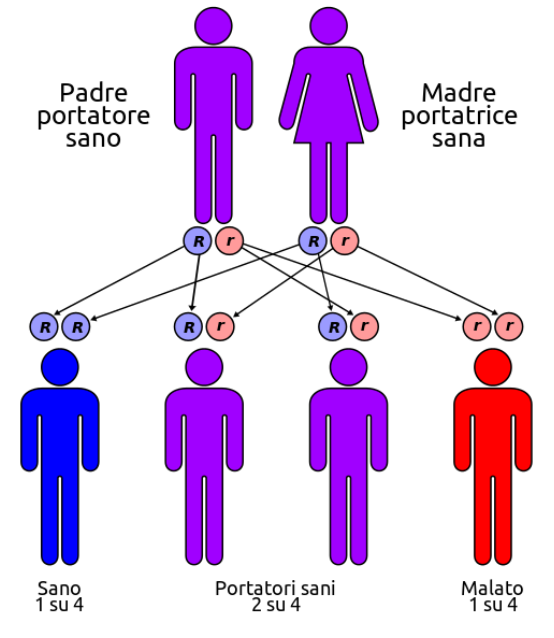
\includegraphics[height=5.5cm, width=4.5cm]{figuraJoubert.jpg}
\end{figure}
Joubert syndrome is a rare genetic disorder that affects the cerebellum, which is the portion of the brain responsible for controlling balance and coordination \cite{1}.
The most common symptoms that indicate the presence of this disease are:
\begin{itemize}
    \item \textbf{ataxia}: loss of muscle coordination;
    \item \textbf{hyperpnea}: increase in the depth of breathing compared to the norm;
    \item \textbf{sleep apnea}: absence of external breathing or pauses in breathing of more than 15 seconds;
    \item abnormal eye and tongue movements;
    \item \textbf{hypotonia}: a reduction in muscle tone of an organ or part of it;
\end{itemize}
Joubert Syndrome is transmitted through an autosomal recessive trait from both parents carriers.\\
 They are generally referred to as "carriers" for individuals who have a given gene, one healthy and one mutated allele, therefore, with the possibility of transmitting a defective allele to her children. \\
In autosomal recessive inheritance, 25\% of children of two heterozygous parents manifest the character and there is the same probability of transmission to both sons at the end that females. \\
The prognosis for this disease is very variable. There are cases where patients have minimal disabilities monotorie but who have a good mental development. However, there are other cases in which individuals have a discrete mental retardation and muscle problems more obvious.\\
Treatment for Joubert syndrome is symptomatic and supportive. In the infant stage it is possible to intervene with stimulation both physical and occupational. Other supportive treatments can affect speech therapy and monitoring of respiration particularly in the neonatal stage. In the absence of a proper diagnosis and appropriate treatment, often leads to death in the second decade of life.

\section{Contribution of the Institute C.S.S. Mendel}
The Institute C.S.S. Mendel is concerned with the study of Joubert syndrome in particular as regards the scope of molecular genetics. Molecular genetics is the field of genetics that focuses on the study of the structure and function of genes at a molecular level. The surveys consist of molecular genetics in the study of DNA and its products, RNA and proteins, whose changes may be related to or responsible for a particular genetic condition. \\
The study of mutation note on Joubert syndrome by sequencing is one of the main objects of research and analysis of the Institute C.S.S. Mendel since 2003 and in recent years has become a European reference center for the study of these syndromes, receiving case studies from around the world and praising numerous collaborations and partnerships \cite{2}.\\
In particular with the assistance of the University of California San Diego, University of Leeds and the Hospital Necker in Paris, researchers from the Instituto CSS Mendel developed a scientific work inherent in a new gene. \\
The study shows that the new gene identified stops the activity of cellular structures-like antennae, called "cilia", which lose their ability to transmit and recognize information both for embryonic development and for the smooth functioning of various organs. 
Joubert syndrome is part of a large group of diseases called "ciliopathies", as the cilia on the cell surface do not follow a proper function is not responding appropriately to the signals. \\
This failure prevents the formation of the embryo proper neural tube, resulting in abnormal development of the central nervous system in children with Joubert syndrome, almost invariably lead to the development of mental retardation of medium to severe. Other anomalies may also affect the retina, the kidneys, the liver and the skeletal system.

\section{Clinical data}
Clinical data that we have been provided by the Institute C.S.S. Mendel relate to an entire sequencing. A sequencing, in the context of molecular biology, is the process of determining the correct order of nitrogenous bases in a nucleic acid. Each sequencing is constituted by a set of samples and each of these is related to a single patient.
A sample has several fields that are divided into an \textit{attributes on the generality of the patient}, an \textit{attributes on specific phenotypic traits of patients} and an \textit{attributes on notes and diagnosis}.\\
The attributes on the generality of the patient are:
\begin{itemize}
   \item \textbf{FAMILY}: family code;
    \item \textbf{NG}: patient code;
    \item \textbf{YOB}: year of born (that we will not consider in queries);
    \item \textbf{last evalutation}  (that we will not consider in queries);
    \item \textbf{sex}: gender of the patient;
    \item \textbf{consang}: presence of consanguineous;
\end{itemize}
Some partial data relating to the attributes on the generality of the patient are:
\begin{figure}[h]
\centering
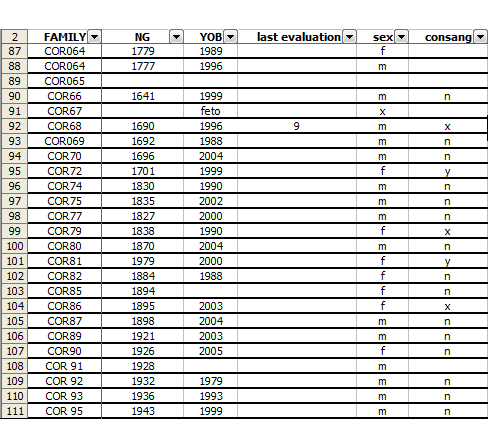
\includegraphics[height=7cm, width=9cm]{attrGeneralitaPaziente.jpg}
\end{figure}
\\
Instead the attributes on specific phenotypic traits of patients are divided on the basis of the main traits and specific characters. 
There are nine main sections and only some of these are analyzed for specific characters. Overall, these are:
\begin{itemize}
   \item \textbf{CNS}: central nervous system;
	\begin{itemize}
      		\item breath;
		\item ID: infectious disease(?);
		\item hypotonia;
		\item ataxia;
		\item apraxia;
		\item nystagmus;
	\end{itemize}
    \item \textbf{eyes};
	\begin{itemize}
      		\item leber amaurosis;
		\item retinopathy;
		\item coloboma;
	\end{itemize}
    \item \textbf{kidneys};
	\begin{itemize}
      		\item renal failure;
		\item NPH: nephronophthisis;
		\item cystis;
		\item eco/blood alterations;
	\end{itemize}
    \item \textbf{liver};
	\begin{itemize}
      		\item eco/blood alterations;
		\item HF: heart failure(?);
	\end{itemize}
    \item \textbf{polydactyly};
	\begin{itemize}
      		\item polydactyly postaxial;
		\item polydactyly mesa-preaxial;
	\end{itemize}
    \item \textbf{tongue};
	\begin{itemize}
      		\item cleft lip/palate;
	\end{itemize}
     \item \textbf{heart};
     \item \textbf{dysmorphic features};
     \item \textbf{MTI}: molar tooth imaging;
	\begin{itemize}
      		\item E/M cele: encepphalo-meningocele;
		\item hydroceph;
      		\item DW: Dandy Walker Malformation;
		\item CC hypopl: Corpus Callosum hypoplasia;
	\end{itemize}
\end{itemize}
Some partial data relating to the attributes on specific phenotypic traits of patients are:
\begin{figure}[hb]
\centering
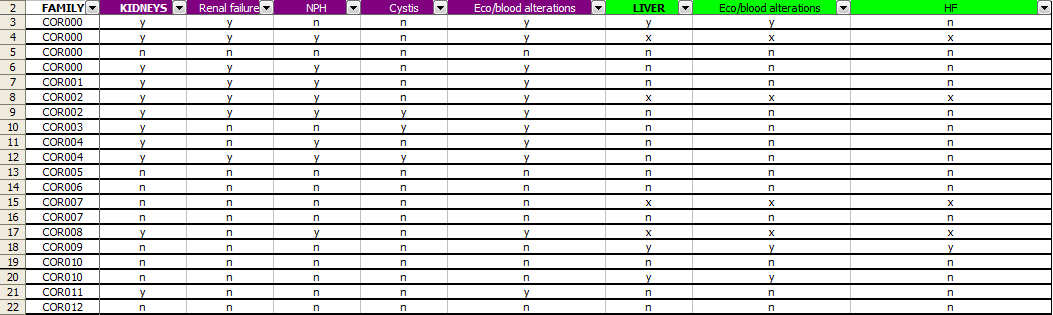
\includegraphics[height=4.2cm, width=14cm]{attrTrattiFenotipici.jpg}
\end{figure}
\\ \\ \\
The last fields of clinical data are additional information and refer to:
\begin{itemize}
   \item notes;
   \item diagnosis;
\end{itemize}
Some partial data relating to the attributes on notes and diagnosis are:
\begin{figure}[hb]
\centering
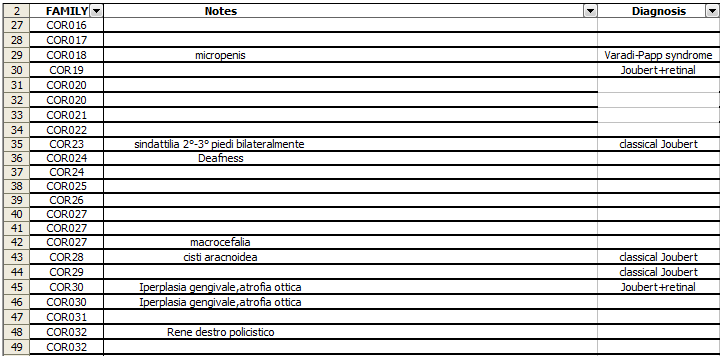
\includegraphics[height=5cm, width=8cm]{attrNotes&Diagnosis.jpg}
\end{figure}

\chapter{Main features of the project}
\section{Aims}
The aim of the project is to create an archive containing people with Joubert Syndrome. This data file consist of the general characteristics of each patient and their phenotypic traits. The main purpose of this archive is to facilitate the association genotype/phenotype of patients under observation at the Institute C.S.S. Mendel. This report make it easier to identify the pathogenetic genetic variants.\\
Each patient manifests different phenotypic traits according to the degree of intensity of the syndrome. People affected by a mild form of the syndrome present problems relating to only some physical components, while patients with more intense forms of the syndrome present the other. The association that is created by the definition of the archive identify the physical components (and hence phenotypic) most relevant to recognize the presence of Joubert Syndrome. \\
The archive is available through a web portal server that allows different interactions with the clinical data of the store. 

\section{Functions}
The portal is used by two types of users:
\begin{itemize}
   \item \textit{admin}: person with the privileges that may adopt measures on the management of the archive;
   \item \textit{simple user}: person who can only use the portal;
\end{itemize}
Based on the user's role distinguish different application functionality. \\
Both types of users can browse the archives through the queries. This function allows users of the portal to view the clinical data on patients who meet the criteria set in the request. In this way, the user sets a query that specifies the parameters that wants to filter. The portal respond to the user by providing the clinical data of individual patients who possess those parameters. The user sees only the general phenotypic characteristics of each patient and then may possibly view traits more specific. In reference to the previous image (mettere numeri alle immagini), the user sees as a possible liver problem, and only then can see that it is particularly eco/blood alteration problem.\\
A simple user can only perform simple queries. An admin user not only uses the portal to search clinical data, but also to perform other operations. Among these features, an admin can:
\begin{itemize}
   \item load clinical data;
	\begin{itemize}
      		\item load an entire sequencing from an Excel file;
		\item load a single sample;
	\end{itemize}
   \item modify existing samples;
\end{itemize}
The admin user has the skills and privileges to interact with the store in a more specific way. This allows him to intervene in the structural details of the store and make decisions about its organization.

\section{Tools}
The development of the project was supported by the use of different tools:
\begin{itemize}
   \item \textbf{PHP}: server-side scripting language designed for web development but also used as a general-purpose programming language \cite{3};
   \item \textbf{Javascript} (JS): dynamic computer programming language \cite{4};
   \item \textbf{Bootstrap}: front-end framework for developing responsive projects on the web \cite{5};
   \item \textbf{Apache HTTP Server}:  web server application \cite{6};
   \item \textbf{MySQL}: open-source relational database management system (RDBMS) \cite{7};
\end{itemize} 
The relevant part of the programming made use of PHP language for writing web interfaces of the portal while JS has been exploited for checking the integrity of the fields of data-entry form or querying. The coding was developed by the \textbf{Eclipse IDE}, adapted of the needs of shared work. For these reasons, the editor was supported by suitable plugin that allowed both writing in the languages mentioned above and the management of the project among the various members of the group.\\
The server side is managed through the use of the Apache HTTP Server, the platform that allows the implementation of the functions of transport and connection information. Web server has permission to provide, by means of dedicated software and user's request, files of any type, such as the web pages of the portal.\\
The management of persistence was finally entrusted to MySQL. This RDBMS allowed to organize in ordered structures clinical data to manage. He also encouraged interaction with the clinical data, facilitating the handling of the queries.


\part{Implementation}

\chapter{Structure}
- da definire-

\chapter{Interface}
- da definire-

\chapter{Model}
- da definire-

\chapter{Persistence}
The management of persistence has been supported by the use of the MySQL RDBMS. Its use has facilitate the operations of interactions with clinical data that make up the data base. In fact, all the features that the portal offers require an exchange of information that requires a collaborative work with persistent data. For this reason all the components involved in the persistence have a close correspondence with the operations that a user can take. We analyze below how we have implemented operations involving the storage and management of data through MySQL.

\section{Setting database}
The organization of information through mySQL has been set so as to corresponding clinical data were provided by Institute C.S.S. Mendel. As shown in figure, we have organized the data in nine tables, one of which is related to patient information, one of these for data administrators while the rest have been introduced in order to handle specific aspects of each character of the observed occurrence of the disease. 
\begin{figure}[h]
\centering
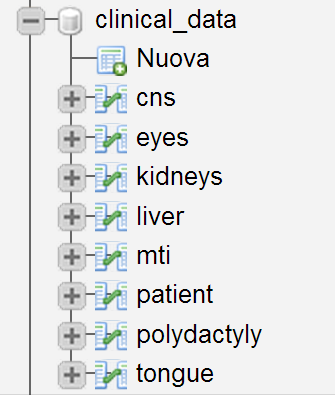
\includegraphics[scale=.35]{db.jpg}
\end{figure}
\\
\textit{Patient} is the entity described by both attributes on the generality of the patient that the attributes on notes and diagnosis. Each tuple of patient entity is characterized by fields (for each attribute is specified the associated type):
\begin{itemize}
      	\item \textbf{ng}  -  int(11);
	\item \textbf{insertionDate} - timestamp;
	\item \textbf{family} - varchar(10);
	\item \textbf{sex} - char(1);
	\item \textbf{consang} - char(1);
	\item \textbf{cns} - char(1);
	\item \textbf{eyes} - char(1);
	\item \textbf{kidneys - char(1)};
	\item \textbf{liver} - char(1);
	\item \textbf{polydactyly} - char(1);
	\item \textbf{tongue} - char(1);
	\item \textbf{heart} - char(1);
	\item \textbf{dysmorphic} - char(1);
	\item \textbf{mti} - char(1);
	\item \textbf{notes} - varchar(300);
	\item \textbf{diagnosis}  - varchar(100);
\end{itemize}
The primary key for the entity \textit{Patient} consists in ng and insertionDate. The attributes related to the physical characteristics (from the cns to mti) that are taken into account in the analysis of the disease, are described  by a single char that can take three values:
\begin{itemize}
	\item y: yes, the patient presents problems for that character observed;
	\item n: no, the patient does not present problems for the character observed;
	\item x or no value: it is not known if the patient develops problems observed for the character;
\end{itemize}
For some of these traits have been observed also create additional entity to manage the specific traits that are affected. These additional tables are available: \textit{CNS}, \textit{Eyes}, \textit{Kidneys}, \textit{Liver}, \textit{MTI}, \textit{Polydactyl} and \textit{Tongue}. Each of these is described by all of the details observed regarding the character of reference, and attributes ng and insertionDate which constitute the primary key. For example, the entity \textit{Eyes} is described by attributes:
\begin{itemize}
	\item \textbf{ng}  -  int(11);
	\item \textbf{insertionDate} - timestamp;
	\item \textbf{leber\_amaurosis} - char(1);
	\item \textbf{retinopathy} - char(1);
	\item \textbf{coloboma} - char(1);
\end{itemize}
In the same way before each specific trait may have values: y,n,x (or no value). \\
The relationships between the different entities are managed by referential constraints between the attributes ng and insertionDate of each tuple.\\ \\
Finally, the entity \textit{Administrators} allows to manage information relating to people authorized to make changes to the database. In particular the tuples of this entity are characterized by attributes only:
\begin{itemize}
	\item \textbf{name}  - varchar(32);
	\item \textbf{password} - varchar(32);
\end{itemize}
These fields form the primary key for the administrator. The presence of this entity is needed to manage authentication of users when using the portal. Only administrative users that have certain privileges can interact with data in a more specific way. It's therefore necessary to be able to detect the user's identity through identification based on username and password. Then an administrator must already be present in the archive.

\subsection{Script}
The script used in mySQL required to define the different entities is partially shown below. There are no reported all the scripts for creating the tables for the characters in which the disease manifests itself; it has been reported that only the entity \textit{Eyes}. The entities missing are generated in a similar way, by modifying the various attributes. \\ \\
\underline{Table structure \textit{Administrator}}
%-------------------------------------------------------------------------------
\begin{flushleft} \small \label{scrap1}
\begin{list}{}{} \item
\mbox{}\verb@CREATE TABLE IF NOT EXISTS `administrators` (@\\
\mbox{}\verb@  `name` varchar(32) NOT NULL,@\\
\mbox{}\verb@  `password` varchar(32) NOT NULL,@\\
\mbox{}\verb@  PRIMARY KEY (`name`,`password`)@\\
\mbox{}\verb@) ENGINE=InnoDB DEFAULT CHARSET=latin1;@\\
\mbox{}\verb@ @\\
\end{list}
\vspace{-1ex}
\footnotesize\addtolength{\baselineskip}{-1ex}
\end{flushleft}
%-------------------------------------------------------------------------------
This entity must necessarily be populated by administrative users. The dump data to the table \textit{Administrator} is:
%-------------------------------------------------------------------------------
\begin{flushleft} \small \label{scrap1}
\begin{list}{}{} \item
\mbox{}\verb@INSERT INTO `administrators` (`name`, `password`) VALUES @\\
\mbox{}\verb@('claudia', 'claudia'),@\\
\mbox{}\verb@('lorenzo', 'lorenzo'),@\\
\mbox{}\verb@('luca', 'luca'),@\\
\mbox{}\verb@('tommaso', 'tommaso');@\\
\mbox{}\verb@ @\\
\end{list}
\vspace{-1ex}
\footnotesize\addtolength{\baselineskip}{-1ex}
\end{flushleft}
%-------------------------------------------------------------------------------
\underline{Table structure \textit{Patient}}
\begin{flushleft} \small \label{scrap1}
\begin{list}{}{} \item
\mbox{}\verb@CREATE TABLE IF NOT EXISTS `patient` ( @\\
\mbox{}\verb@  `ng` int(11) NOT NULL,@\\
\mbox{}\verb@  `insertion_date` timestamp NOT NULL DEFAULT CURRENT_TIMESTAMP @\\
\mbox{}\verb@      ON UPDATE CURRENT_TIMESTAMP,@\\
\mbox{}\verb@  `family` varchar(10) NOT NULL,@\\
\mbox{}\verb@  `sex` char(1) NOT NULL,@\\
\mbox{}\verb@  `consang` char(1) NOT NULL,@\\
\mbox{}\verb@  `cns` char(1) NOT NULL,@\\
\mbox{}\verb@  `eyes` char(1) NOT NULL,@\\
\mbox{}\verb@  `kidneys` char(1) NOT NULL,@\\
\mbox{}\verb@  `liver` char(1) NOT NULL,@\\
\mbox{}\verb@  `polydactyly` char(1) NOT NULL,@\\
\mbox{}\verb@  `tongue` char(1) NOT NULL,@\\
\mbox{}\verb@  `heart` char(1) NOT NULL,@\\
\mbox{}\verb@  `dysmorphic` char(1) NOT NULL,@\\
\mbox{}\verb@  `mti` char(1) NOT NULL,@\\
\mbox{}\verb@  `notes` varchar(300) NOT NULL,@\\
\mbox{}\verb@`diagnosis` varchar(100) NOT NULL,@\\
\mbox{}\verb@  PRIMARY KEY (`ng`,`insertion_date`)@\\
\mbox{}\verb@) ENGINE=InnoDB DEFAULT CHARSET=latin1;@\\
\mbox{}\verb@ @\\
\end{list}
\vspace{-1ex}
\footnotesize\addtolength{\baselineskip}{-1ex}
\end{flushleft}
%-------------------------------------------------------------------------------
\underline{Table structure \textit{Eyes}}
\begin{flushleft} \small \label{scrap1}
\begin{list}{}{} \item
\mbox{}\verb@CREATE TABLE IF NOT EXISTS `eyes` ( @\\
\mbox{}\verb@  `ng_eyes` int(11) NOT NULL,@\\
\mbox{}\verb@  `insertion_date_eyes` timestamp NOT NULL DEFAULT CURRENT_TIMESTAMP @\\
\mbox{}\verb@      ON UPDATE CURRENT_TIMESTAMP,@\\
\mbox{}\verb@  `leber_amaurosis` char(1) NOT NULL,@\\
\mbox{}\verb@  `retinopathy` char(1) NOT NULL,@\\
\mbox{}\verb@  `coloboma` char(1) NOT NULL,@\\
\mbox{}\verb@  PRIMARY KEY (`ng_eyes`,`insertion_date_eyes`)@\\
\mbox{}\verb@) ENGINE=InnoDB DEFAULT CHARSET=latin1;@\\
\mbox{}\verb@ @\\
\end{list}
\vspace{-1ex}
\footnotesize\addtolength{\baselineskip}{-1ex}
\end{flushleft}
%-------------------------------------------------------------------------------



\section{Loading data}
Loading data into the database follows the two modes provided by the functions that the portal offers the user: load a single sample or load an entire sequencing.

\subsection{Loading of a single sample}
An admin user can upload data is related to a whole load sequencing both the individual samples. Analyze below the two different loading modes.\\
It was initially defined a class \textit{LoadRecord} inside of which have been implemented methods that allow the loading of a single sample associated with a single patient. In particular the \textit{Load} function is responsible for defining the SQL strings that allow the rescue of the various fields of each table. \\
This function has allowed to define the set of attributes, that must manage to analyze the syndrome, in a data structure:
%-------------------------------------------------------------------------------
\begin{flushleft} \small \label{scrap1}
\begin{list}{}{} \item
\mbox{}\verb@public static function Load( $record, $row=1) { @\\ 
\mbox{}\verb@ @\\
\mbox{}\verb@	$lr = new LoadRecord();@\\
\mbox{}\verb@	$record = $lr->insertX($record);@\\
\mbox{}\verb@ @\\
\mbox{}\verb@	$log = new Log();@
\mbox{}\verb@ @\\
\mbox{}\verb@ list($FAMILY, $NG, $YOB, $last_evaluation, $sex, $consang, @\\
\mbox{}\verb@      $CNS, $breath, $id, $hypotonia, $ataxia, $apraxia, $nystagmus,@\\
\mbox{}\verb@      $EYES, $leber_amaurosis, $retinopathy, $coloboma,@\\
\mbox{}\verb@      $KIDNEYS, $renal_failure, $nph, $Cystis, $eco_blood_alterations,@\\
\mbox{}\verb@      $LIVER, $eco_blood_alterations_liver, $hf, @\\
\mbox{}\verb@      $POLYDACTYLY, $postaxial, $mesa_preaxial,@\\
\mbox{}\verb@      $TONGUE, $cleft_lip_palate, $HEART, $DYSMORPHIC_FEATURES,@\\
\mbox{}\verb@      $MTI, $em_cele, $hydroceph, $dw, $cc_hypopl, $Notes, $Diagnosis) = $record;@\\
\mbox{}\verb@ @\\
\mbox{}\verb@      $success = 0;@\\
\mbox{}\verb@ @\\
\mbox{}\verb@      if($NG != null && is_numeric($NG)){	@\\
\mbox{}\verb@         $mysqli = new mysqli('localhost', 'root', '', 'clinical_data');@\\
\mbox{}\verb@         $mysqli->autocommit(true);@\\	
\mbox{}\verb@ @\\
\mbox{}\verb@         date_default_timezone_set("Europe/Rome");@\\
\mbox{}\verb@         //$insertion_date = date("Y-m-d H:i:s");@\\
\mbox{}\verb@         $insertion_date = date("Y-m-d");@\\
\mbox{}\verb@ @\\
\mbox{}\verb@         //riempie tabella patient@\\
\mbox{}\verb@ @\\
\mbox{}\verb@         //ATTENZIONE OVVIAMENTE NON VA BENE COSI', HO RISOLTO IL PROBLEMA TOGLIENDO LE NOTE@\\
\mbox{}\verb@         if($NG == 1936)@\\
\mbox{}\verb@            $Notes = "";@\\
\mbox{}\verb@ @\\
\end{list}
\vspace{-1ex}
\footnotesize\addtolength{\baselineskip}{-1ex}
\end{flushleft}
%-------------------------------------------------------------------------------

In the same function have also been defined SQL statements for the composition of the database.\\
In this way it was implemented the inclusion of information relating to patients:
%-------------------------------------------------------------------------------
\begin{flushleft} \small \label{scrap1}
\begin{list}{}{} \item
\mbox{}\verb@        $query= sprintf("INSERT INTO patient (ng, insertion_date, @\\
\mbox{}\verb@            family, sex, consang, cns, eyes, kidneys, liver, polydactyly,  @\\
\mbox{}\verb@            tongue, heart, dysmorphic, mti, notes, diagnosis) VALUES@\\
\mbox{}\verb@            (' %s', '%s', '%s','%s', '%s', '%s','%s', '%s','%s','%s', '%s',@\\
\mbox{}\verb@             '%s','%s', '%s', '%s','%s')",$NG."ciao",$insertion_date,$FAMILY,@\\
\mbox{}\verb@            $sex,$consang,$CNS,$EYES,$KIDNEYS,$LIVER,$POLYDACTYLY,@\\
\mbox{}\verb@            $TONGUE,$HEART,$DYSMORPHIC_FEATURES,$MTI,$Notes,$Diagnosis);@\\
\mbox{}\verb@ @\\
\mbox{}\verb@            $dati=$mysqli->query($query);@\\
\mbox{}\verb@            if($dati) {@\\
\mbox{}\verb@               $success++;         @\\
\mbox{}\verb@            }            @\\
\mbox{}\verb@            else {            @\\
\mbox{}\verb@               $log->write( "fallimentoPatient riga: $row" . "<br />");         @\\
\mbox{}\verb@            }@\\
\mbox{}\verb@ @\\
\end{list}
\vspace{-1ex}
\footnotesize\addtolength{\baselineskip}{-1ex}
\end{flushleft}
%-------------------------------------------------------------------------------

In a similar way we have defined the inclusion of detailed clinical data relating to the main aspects of the disease:
%-------------------------------------------------------------------------------
\begin{flushleft} \small \label{scrap1}
\begin{list}{}{} \item
\mbox{}\verb@            if($success > 0) { @\\
\mbox{}\verb@               $query= sprintf("INSERT INTO cns(ng_cns, insertion_date_cns, @\\
\mbox{}\verb@               breath, id, hypotonia, ataxia, apraxia, nystagmus) VALUES@\\
\mbox{}\verb@               ('%s', '%s', '%s', '%s', '%s', '%s', '%s', '%s')",$NG, $insertion_date,@\\
\mbox{}\verb@               $breath , $id, $hypotonia, $ataxia, $apraxia, $nystagmus);@\\
\mbox{}\verb@ @\\
\mbox{}\verb@             $dati=$mysqli->query($query);@\\
\mbox{}\verb@             if($dati) {@\\
\mbox{}\verb@                $success++;         @\\
\mbox{}\verb@             }            @\\
\mbox{}\verb@             else {            @\\
\mbox{}\verb@                $log->write( "fallimentoCNS riga: $row" . "<br />");         @\\
\mbox{}\verb@             [...] @\\
\mbox{}\verb@            }@\\
\mbox{}\verb@       $mysqli->close();@\\
\mbox{}\verb@ @\\
\end{list}
\vspace{-1ex}
\footnotesize\addtolength{\baselineskip}{-1ex}
\end{flushleft}
%-------------------------------------------------------------------------------
In the [...] we proceeded in the same way to the management of data entry for the other generic aspects.

\subsection{Loading of an entire sequencing}
The portal also offers the ability to upload a sequencing that allows to insert into the database multiple samples simultaneously. These samples need to be collected in an Excel file according to a specific pattern of the composition of attributes. The interaction between the portal and the management of data via Excel spreadsheet was supported by \textbf{PHPExcel}. \\
PHPExcel is a "\textit{Project providing a set of classes for the PHP programming language, which allow you to write to and read from different spreadsheet file formats, like Excel (BIFF) .xls, Excel 2007 (OfficeOpenXML) .xlsx, CSV, Libre/OpenOffice Calc .ods, Gnumeric, PDF, HTML, ... This project is built around Microsoft's OpenXML standard and PHP}"\cite{n}. It is a library that has facilitated the reading of the Excel input file and allowed to extrapolate from these clinical and general information for the definition of the database. His contribution has been exploited in the class \textit{Read Excel} in which the \textit{Read} method was responsible for the loading the file:
%-------------------------------------------------------------------------------
\begin{flushleft} \small \label{scrap1}
\begin{list}{}{} \item
\mbox{}\verb@public static function Read($path) {@\\
\mbox{}\verb@   try {@\\
\mbox{}\verb@      $inputFileType = PHPExcel_IOFactory::identify($path);@\\
\mbox{}\verb@      $objReader = PHPExcel_IOFactory::createReader($inputFileType);@\\
\mbox{}\verb@      $objPHPExcel = $objReader -> load($path);@\\
\mbox{}\verb@   } catch (Exception $e) {@\\
\mbox{}\verb@      die('Error loading file "' . pathinfo($path, @\\
\mbox{}\verb@      PATHINFO_BASENAME) . '":' . $e -> getMessage());@\\
\mbox{}\verb@   }@\\
\mbox{}\verb@ @\\
\mbox{}\verb@      //  Get worksheet dimensions@\\
\mbox{}\verb@   $sheet = $objPHPExcel -> getSheet(0);@\\
\mbox{}\verb@   $highestRow = $sheet -> getHighestRow();@\\
\mbox{}\verb@   $highestColumn = $sheet -> getHighestColumn();@\\
\mbox{}\verb@ @\\
\mbox{}\verb@   $rowAdd = 0;@\\
\mbox{}\verb@   for ($row = 2; $row <= $highestRow; $row++) {@\\
\mbox{}\verb@      //  Read a row of data into an array@\\
\mbox{}\verb@      $rowData = $sheet -> rangeToArray('A' . $row . ':' .@\\
\mbox{}\verb@      $highestColumn . $row, NULL, TRUE, FALSE);@\\
\mbox{}\verb@ @\\
\mbox{}\verb@      $loadRecord = new LoadRecord();@\\
\mbox{}\verb@      $rowAdd += $loadRecord->load($rowData[0],$row);@\\
\mbox{}\verb@   }@\\
\mbox{}\verb@ @\\
\mbox{}\verb@   return $rowAdd;@\\
\mbox{}\verb@}@\\
\end{list}
\vspace{-1ex}
\footnotesize\addtolength{\baselineskip}{-1ex}
\end{flushleft}
%-------------------------------------------------------------------------------

Within this function has been taken over the previously described method. In this way, the loading of a entire sequencing  invokes the method \textit{LoadRecord} for loading a single sample.\\ 
The function \textit {Read} takes as a parameter the path of traceability of the excel file to be loaded. An application of this function is shown in the class \textit{FromExcelToDB} in which is set the loading data: 
%-------------------------------------------------------------------------------
\begin{flushleft} \small \label{scrap1}
\begin{list}{}{} \item
\mbox{}\verb@$log = new Log();@\\
\mbox{}\verb@$log->emptyAll();@\\
\mbox{}\verb@ @\\
\mbox{}\verb@$path = 'db_clinico.xlsx';@\\
\mbox{}\verb@$readExcel = new ReadExcel();@\\
\mbox{}\verb@$recordAdd = $readExcel->read($path);@\\
\mbox{}\verb@ @\\
\mbox{}\verb@echo ("Sono stati aggiunti $recordAdd record" . "<br />");@\\
\mbox{}\verb@ @\\
\mbox{}\verb@echo ($log->read());@\\
\mbox{}\verb@ @\\
\end{list}
\vspace{-1ex}
\footnotesize\addtolength{\baselineskip}{-1ex}
\end{flushleft}
%-------------------------------------------------------------------------------
In this case, \textit{'db\_clinico.xlsx'} represents our input excel file to be loaded into the database.


 
\cleardoublepage
\begin{thebibliography}{8}
\bibitem{1} http://en.wikipedia.org/wiki/Joubert syndrome;
\bibitem{2} http://www.css-mendel.it/ricerca/sindrome di joubert/
\bibitem{3} http://en.wikipedia.org/wiki/PHP;
\bibitem{4} http://en.wikipedia.org/wiki/Javascript;
\bibitem{5} http://getbootstrap.com/;
\bibitem{6} http://en.wikipedia.org/wiki/Apache HTTP Server;
\bibitem{7} http://en.wikipedia.org/wiki/MySQL;
\bibitem{n} https://phpexcel.codeplex.com/;
\end{thebibliography}

\end{document}
